% !TeX TXS-program:compile = txs:///lualatex

\documentclass[a4paper,11pt]{article}
\usepackage[revgoku]{cp-base}
\graphicspath{{./graphics/}}
%variables
\donnees[%
	classe={1\up{ère} 2M2},matiere={[SPÉ.MATHS]},mois=Mars,annee=2022,typedoc=CHAP,numdoc=8
]
%formatage
\author{Pierquet}
\title{\nomfichier}
\hypersetup{pdfauthor={Pierquet},pdftitle={\nomfichier},allbordercolors=white,pdfstartview=FitH}
%divers
\lhead{\entete{\matiere}}
\chead{\entete{\lycee}}
\rhead{\entete{\classe{} - \mois{} \annee}}
%\rhead{\entete{\classe{} - Chapitre }}
\lfoot{\pied{\matiere}}
\cfoot{\logolycee{}}
\rfoot{\pied{\numeropagetot}}
\intervalconfig{separator symbol=;}

\begin{document}
	
\pagestyle{fancy}

\part{CH08 - Fonctions dérivées - Exercices (correction)}

\exonum{0}

\begin{enumerate}
	\item On a $f(3)=3^3 + 3^2 + 3 + 1 = 40$.
	\item
	\begin{enumerate}
		\item La fonction $f$ est dérivable sur $\R$ et $f'(x)=3x^2+2x+1$.
		\item Ainsi on a $f'(3)= 3 \times 3^2 + 2 \times 3 + 1 = 34$.
		\item Une équation de $\mathscr{T}_3$ est $y=f'(3) \times (x-3) + f(3) = 34 \times (x+2) + 40 = 34x-102+40=34x-62$.
	\end{enumerate}
	\item De même une équation de $\mathscr{T}_{-1}$ est $y=f'(-1) \times (x-(-1)) + f(-1) = 2 \times (x+1) + 0=2x+2$.
	
	Avec $\begin{dcases}f(-1)=(-1)^3+(-1)^2+(-1)+1=0 \\ f'(-1)=3 \times (-1)^2+2 \times (-1)+1=2 \end{dcases}$.
\end{enumerate}

\medskip

\exonum{1}

\begin{enumerate}
	\item La \ccalg{calculatrice} nous suggère que $f'(4)=\dfrac{15}{16}$ avec $f(x)=x+\dfrac{1}{x}$.
	
	En effet, on a $f'(x)=1-\dfrac{1}{x^2}$ de sorte que $f'(4)=1-\dfrac{1}{4^2}=1-\dfrac{1}{16}=\dfrac{16}{16}-\dfrac{1}{16}=\dfrac{15}{16}$ $\checked$.
	\item Le logiciel \cxcas{Xcas} nous suggère que $f'(5) \approx 2,23606797$ avec $f(x)=10\sqrt{x}$.
	
	En effet, on a $f'(x)=10 \times \dfrac{1}{2\sqrt{x}}=\dfrac{5}{\sqrt{x}}$ de sorte que $f'(5)=\dfrac{5}{\sqrt{5}}=\sqrt{5} \approx 2,23606797$ $\checked$.
\end{enumerate}

\medskip

\exonum{1}

\begin{enumerate}
	\item 
	\begin{enumerate}
		\item $f(x)=2x^3+4x^2-5x+6$ est dérivable sur $\R$ et $f'(x)=2 \times 3x^2 + 4 \times 2x -5 = 6x^2+8x-5$.
		\item $g(x)=5x+\dfrac{2}{x}$ est dérivable sur $\R^*$ et $g'(x)=5 + 2 \times \dfrac{-1}{x^2} = 5-\dfrac{2}{x^2}$.
		\item $h(x)=4\sqrt{x}-7x$ est dérivable sur $\intervOO{0}{+\infty}$ et $h'(x)=4 \times \dfrac{1}{2\sqrt{x}} - 7 = \dfrac{2}{\sqrt{x}}-7$.
	\end{enumerate}
	\item 
	\begin{enumerate}
		\item Une équation de $\mathscr{T}_2$ est $y=f'(2) \times (x-2)+f(2)=35 \times (x-2) + 28 = 35x-70+28=35x-42$.
		
		Avec $\begin{dcases}f(2)=2 \times 2^3+4 \times 2^2 - 5 \times 2 +6 = 35 \\ f'(2)=6 \times 2^2+8 \times 2-5=28 \end{dcases}$.
		\item Une équation de $\mathscr{T}_{-1}$ est $y=g'(-1) \times (x-(-1)) + g(-1) = 3 \times (x+1) + (-7) = 3x+3-7=3x-4$.
		
		Avec $\begin{dcases}g(-1)=5 \times (-1) + \dfrac{2}{-1} = -7 \\ g'(-1)=5 -\dfrac{2}{(-1)^2}=3 \end{dcases}$.
		\item Une équation de $\mathscr{T}_9$ est $y=h'(9) \times (x-9)+h(9) = -\dfrac{19}{3} \times (x-9) + (-51) = -\dfrac{19}{3}x+6$.
		
		Avec $\begin{dcases}h(9)=4 \times \sqrt{9} - 7 \times 9 = 12-63 = -51 \\ h'(9)=\dfrac{2}{\sqrt{9}}-7 = \dfrac{2}{3} - 7 = -\dfrac{19}{3} \end{dcases}$.
	\end{enumerate}
\end{enumerate}

\newpage

\exonum{2}

\begin{enumerate}
	\item La fonction $f$ est un produit $u \times v$ avec :
	
	\tabula{}$\begin{dcases}u=x^2+1 \\ v=-x^3+2x^2+5\end{dcases}$ et $\begin{dcases}u'=2x \\ v'=3x^2+4x\end{dcases}$.
	
	Ainsi $f'(x)=u'v+v'u=2x \times \big(-x^3+2x^2+5\big) + \big(3x^2+4x\big) \times \big( x^2+1 \big)$ pour tout réel $x$.
	\item La fonction $g$ est un produit $u \times v$ avec :
	
	\tabula{}$\begin{dcases}u=x+1 \\ v=\sqrt{x}\end{dcases}$ et $\begin{dcases}u'=1 \\ v'=\tfrac{1}{2\sqrt{x}}\end{dcases}$.
	
	Ainsi $g'(x)=u'v+v'u=1 \times \sqrt{x} +  \dfrac{1}{2\sqrt{x}} \times (x+1) = \sqrt{x} + \dfrac{x+1}{2\sqrt{x}} = \dfrac{\sqrt{x} \times 2\sqrt{x} + (x+1)}{2\sqrt{x}} = \dfrac{2x+x+1}{2\sqrt{x}}=\dfrac{3x+1}{2\sqrt{x}}$.
	\item La fonction $h$ s'écrit sous forme d'un quotient $\tfrac{u}{v}$ avec :
	
	\tabula{}$\begin{dcases}u=3x+1 \\ v=x-5\end{dcases}$ et $\begin{dcases}u'=3 \\ v'=1\end{dcases}$.
	
	Ainsi $h'(x)=\dfrac{u'v-v'u}{v^2} = \dfrac{3 \times (x-5) - 1 \times (3x+1)}{(x-5)^2}=\dfrac{3x-15-3x-1}{(x-5)^2}=\dfrac{-16}{(x-5)^2}$ pour $x \neq 5$.
	\item La fonction $k$ s'écrit avec une somme et un quotient :
	
	\tabula{}$(2x)'=2$ et $\left( \dfrac{2}{x^2+1} \right)^{\prime} = \dfrac{0 \times \big(x^2+1\big)-2x \times 1}{\big(x^2+1\big)^2}=\dfrac{-2x}{\big(x^2+1\big)^2}$.
	
	Ainsi $k'(x)=2 + \dfrac{-2x}{\big(x^2+1\big)^2} = \dfrac{2 \times \big(x^2+1\big)^2-2x}{\big(x^2+1\big)^2} = \dfrac{2x^4+4x^2+2-2x}{\big(x^2+1\big)^2} = \dfrac{2x^4+4x^2-2x+2}{\big(x^2+1\big)^2}$ pour tout $x$.
\end{enumerate}

\medskip

\exonum{3}

\begin{enumerate}
	\item $f(x)=(3x+1)^3$ est sous la forme  $u^3$ avec $u=3x+1$ et donc $u'=3$.
	
	On a donc $f'(x)=3 \times u' \times u^2 = 3 \times 3 \times (3x+1)^2=9(3x+1)^2$ pour tout $x$.
	\item $g(x)=\sqrt{2x+1}$ est sous la forme $\sqrt{u}$ avec $u=2x+1$ et donc $u'=2$.
	
	On a donc $g'(x)=\dfrac{u'}{2\sqrt{u}}=\dfrac{2}{2\sqrt{2x+1}}=\dfrac{1}{\sqrt{2x+1}}$ pour tout $x >-0,5$.
	\item $h(x)=\sqrt{x-2}\,\big(x^2-1\big)$ est sous forme d'un produit :
	
	\tabula{}$u=\sqrt{x-2}$ qui donne $u'=\dfrac{(x-2)'}{2\sqrt{x-2}}=\dfrac{1}{2\sqrt{x-2}}$ et $v=x^2-1$ qui donne $v'=2x$.
	
	On a donc $g'(x)=\dfrac{1}{2\sqrt{x-2}} \times \big(x^2-1\big) + 2x \times \sqrt{x-2}$ pour tout $x >2$.
\end{enumerate}

\medskip

\exonum{2}

\begin{enumerate}
	\item La fonction $f$ est dérivable sur $\intervFF{0}{7}$ et $f'(x)=3x^2 - 11 \times 2x + 39$.
	\item $f'(x)$ est un trinôme du second degré, on utilise donc $\Delta$ :
	
	\tabula{}$\Delta = (-22)^2 - 4 \times 3 \times 39 = 4$ et donc $\begin{dcases} x_1=\tfrac{-(-22)+\sqrt{16}}{2 \times 3} = \tfrac{22+4}{6}=\tfrac{13}{3} \\ x_2=\tfrac{-(-22)-\sqrt{16}}{2 \times 3} = \tfrac{22-4}{6}=3 \end{dcases}$ et le signe de $a=3$ est positif.
	
	Ainsi on a :
	\begin{center}
		\begin{tikzpicture}
			\tkzTabInit{$x$/0.8,$f'(x)$/0.8}{$0$,$3$,$\tfrac{13}{3}$,$7$}
			\tkzTabLine{,+,z,-,z,+,}
		\end{tikzpicture}
	\end{center}
	\item D'après les \og travaux \fg{} du chapitre 07, on peut dire que :
	\begin{itemize}
		\item sur $\intervFF{0}{3}$, la fonction $f$ est croissante ;
		\item sur $\intervFF{3}{\tfrac{13}{3}}$, la fonction $f$ est décroissante ;
		\item sur $\intervFF{\tfrac{13}{3}}{7}$, la fonction $f$ est croissante.
	\end{itemize}
\end{enumerate}

\medskip

\exonum{3}

\begin{enumerate}
	\item Les éventuelles valeurs interdites de $f$ sont les racines de $4x^2+4x+5$.
	
	Or $\Delta=-64$, donc le dénominateur ne s'annule pas, ce qui justifie que $f$ est définie sur $\R$.
	\item La fonction $f$ est dérivable sur $\R$ et s'écrit sous forme d'un quotient avec :
	
	\tabula{}$\begin{dcases}u=2x+1 \\ v=4x^2+4x+5\end{dcases}$ et $\begin{dcases}u'=2 \\ v'=8x+4\end{dcases}$.
	
	Ainsi $f'(x)=\dfrac{u'v-v'u}{v^2}=\dfrac{2 \times \big(4x^2+4x+5\big)- (8x+4) \times (2x+1)}{\big(4x^2+4x+5\big)^2}$.
	
	Soit encore $f'(x) = \dfrac{8x^2+8x+10-16x^2-8x-8x-4}{\big(4x^2+4x+5\big)^2} = \dfrac{-8x^2-8x+6}{\big(4x^2+4x+5\big)^2}$ pour tout $x$.
	\item La fonction $f'(x)$ est bien sous forme de quotient :
	\begin{itemize}
		\item le dénominateur est le carré d'une expression ne s'annulant jamais, donc il est strictement positif ;
		\item le numérateur est un trinôme, donc $\Delta=256$ qui donne $\begin{dcases} x_1 = -1,5 \\ x_2 = 0,5 \end{dcases}$ avec $a=-8$ négatif.
	\end{itemize}
	\begin{center}
		\begin{tikzpicture}
			\tkzTabInit{$x$/0.8,NUM/0.8,DÉNOM/0.8,$f'(x)$/0.8}{$-\infty$,${-1,5}$,${0,5}$,$+\infty$}
			\tkzTabLine{,-,z,+,z,-,}
			\tkzTabLine{,+,t,+,t,+,}
			\tkzTabLine{,-,z,+,z,-,}
		\end{tikzpicture}
	\end{center}
	\item D'après les \og travaux \fg{} du chapitre 07, on peut dire que :
	\begin{itemize}
		\item sur $\intervOF{-\infty}{-1,5}$, la fonction $f$ est décroissante ;
		\item sur $\intervFF{-1,5}{0,5}$, la fonction $f$ est croissante ;
		\item sur $\intervFO{0,5}{+\infty}$, la fonction $f$ est décroissante.
	\end{itemize}
	\item La seule courbe \og compatible \fg{} avec les variations précédentes est :
	\begin{center}
		\tunits{0.8}{8}
		\tdefgrille{-3}{3}{1}{0.5}{-0.301}{0.3}{0.1}{0.05}
		\begin{tikzpicture}[x=\xunit cm,y=\yunit cm]
			\tgrilles[line width=0.35pt,lightgray] ; \axestikz*[width=0.75pt] ;
			\axextikz[width=0.75pt,size=\scriptsize]{-3,-2,...,2} ; \axeytikz[width=0.75pt,size=\scriptsize]{-0.3,-0.2,-0.1,0,0.1,0.2} ;
			\draw[very thick,red,domain=\xmin:\xmax,samples=250] plot (\x,{(2*\x+1)/(4*\x*\x+4*\x+5)}) ;
			\draw[thick,blue,densely dotted] (-1.5,0) -- (-1.5,-0.25) (0.5,0) -- (0.5,0.25) ;
			\filldraw[blue] (-1.5,-0.25) circle[radius=2pt] (0.5,0.25) circle[radius=2pt] ;
			\draw (2,0.215) node[red] {\large $\mathscr{C}_f$} ;
		\end{tikzpicture}
	\end{center}
\end{enumerate}

\end{document}